%% ===================================================================
%%  Village Pond Planning System (Terrain Analyzer)
%%  ACM SIGCONF / SIGAPP-style technical report
%%
%%  All quantitative claims in this document were derived by direct
%%  inspection and execution of the repository at commit 25284a7 and by
%%  the reproducible measurement scripts described in Section 5.1.
%%
%%  Compiled with Tectonic (XeTeX) using acmart sigconf in review mode.
%%  The author name below is taken from the repository commit metadata; no
%%  institutional affiliation, postal address or e-mail was available in the
%%  source material, and none has been invented here.
%% ===================================================================

\documentclass[sigconf,review,10pt]{acmart}

\AtBeginDocument{%
  \providecommand\BibTeX{{Bib\TeX}}}

\usepackage{booktabs}
\usepackage{array}
\usepackage{multirow}
\usepackage{graphicx}
\usepackage{amsmath}
\usepackage{url}
\usepackage{balance}
\usepackage{tikz}
\usetikzlibrary{positioning,arrows.meta,fit,calc,shapes.geometric,backgrounds}
%% Character protrusion lets narrow ACM columns justify text without
%% overfull boxes; this is the standard remedy for long unbreakable
%% identifiers in two-column proceedings. acmart already loads microtype,
%% so features are selected with \microtypesetup rather than package
%% options, which would raise an option clash. Font expansion is disabled
%% because this document is compiled with XeTeX via Tectonic, and expansion
%% is not supported there.
\usepackage{microtype}
\microtypesetup{protrusion=true,expansion=false}
%% Emergency stretch is the last-resort glue TeX may call on before it
%% reports an overfull box. Without it, paragraphs containing long
%% identifiers exceed the measure and the offending text overruns the
%% neighbouring column.
\setlength{\emergencystretch}{3em}
\hbadness=10000

%% Ragged-right paragraph column: long unbreakable identifiers are common in
%% this document, and a justified p-column reports them as overfull boxes.
\newcolumntype{R}[1]{>{\raggedright\arraybackslash}p{#1}}
%% Long monospaced identifiers and file paths appear throughout this
%% document. Without explicit break opportunities TeX reports them as
%% overfull boxes, so \cb (a zero-width penalty permitting a line break) is
%% inserted after every path and word separator inside them.
\newcommand{\cb}{\allowbreak}
\newcommand{\codelong}[1]{\texttt{#1}}

%% ---------------------------------------------------------------------
%%  Author block
%% ---------------------------------------------------------------------
\author{Abhigyan Sharma}

\begin{document}

\title{Village Pond Planning System: A Terrain-Driven Web GIS for
Siting Farm Ponds from Survey Contours and Open Elevation Data}

\begin{abstract}
Smallholder farmers in rain-fed agricultural regions frequently identify
farm pond sites from visual inspection alone, a practice that discards
information already encoded in published topographic survey sheets. This
paper presents Terrain Analyzer, a containerised web GIS that converts
survey contour maps, delivered as KML or KMZ files, into a quantitative,
ranked recommendation for farm pond siting. The system reconstructs a
digital elevation model (DEM) from vector contour lines by Delaunay
triangulation with linear interpolation inside the convex hull and inverse
distance weighting outside it, then derives slope, aspect, D8 flow
direction, flow accumulation, depression depth and delineated catchment
boundaries. A five-criterion weighted composite score combines terrain
slope, natural depression depth, upstream catchment, relative elevation
and long-term rainfall, after which deterministic candidate selection
enforces spatial separation and excludes watercourses. Historical
precipitation is retrieved from the Open-Meteo archive and converted to a
seasonal runoff volume through the runoff coefficient method. We report a
27-operation REST interface served by FastAPI with a React and Leaflet
client, and a fully automated test suite of 102 passing cases. On a
1,355-contour, 6.71~MB survey sheet spanning 267--298~m elevation, the
end-to-end reconstruction, scoring and delineation pipeline completes in
242--277~ms (median 260~ms) and returns a rank-1 site scoring 43.1/100.
We release the design, the algorithms, the measured performance envelope
and an explicit statement of the engineering decisions and current
defects that remain before the tool can support construction decisions.
\end{abstract}

\begin{CCSXML}
<ccs2012>
  <concept>
    <concept_id>10011007.10011074</concept_id>
    <concept_desc>Software and its engineering~Software creation and management</concept_desc>
    <concept_significance>500</concept_significance>
  </concept>
  <concept>
    <concept_id>10011007.10011074.10011084</concept_id>
    <concept_desc>Software and its engineering~Software development methodologies</concept_desc>
    <concept_significance>500</concept_significance>
  </concept>
  <concept>
    <concept_id>10010147.10010257</concept_id>
    <concept_desc>Earth and environmental sciences~Hydrology</concept_desc>
    <concept_significance>500</concept_significance>
  </concept>
  <concept>
    <concept_id>10010147.10010241.10010242.10010243</concept_id>
    <concept_desc>Earth and environmental sciences~Water resources management</concept_desc>
    <concept_significance>500</concept_significance>
  </concept>
  <concept>
    <concept_id>10003120.10003121</concept_id>
    <concept_desc>Human-centered computing~Human computer interaction (HCI)</concept_desc>
    <concept_significance>300</concept_significance>
  </concept>
</ccs2012>
\end{CCSXML}

\keywords{digital elevation model, terrain analysis, farm pond siting,
geographic information system, D8 flow routing, suitability analysis,
web GIS, FastAPI, Leaflet}

\maketitle

%% ===================================================================
\section{Introduction}
%% ===================================================================

\subsection{Motivation}

Water harvesting ponds are the principal on-farm water security
infrastructure in rain-fed agriculture. Siting such a pond is a
compromise between several competing objectives: a gently sloping
construction footprint limits earthworks, a genuine topographic depression
minimises excavation, a large upstream catchment supplies water, and a low
relative elevation enables gravity-fed withdrawal. Farmers and extension
officers typically balance these criteria by eye, walking the field and
judging slope and drainage from experience. The material cost of a poor
choice is substantial: a pond sited on a throughflow channel either
fails to hold water or is scoured, and a pond sited on a ridge crest
captures no runoff at all.

The topographic information required to make this decision objectively is
frequently already in existence. Government survey departments publish
contour sheets at 1~m or 2~m intervals, and these sheets are increasingly
distributed as KML or KMZ vector files for use in consumer mapping
software. This information is rarely exploited for farm pond planning.
The work reported here closes that gap: it treats a published contour
sheet as the primary data source and returns a ranked, quantitatively
justified pond site together with its upstream catchment.

\subsection{Contributions}

This paper describes a complete, running system rather than an isolated
algorithm. Its contributions are:

\begin{enumerate}
  \item A contour-to-DEM reconstruction pipeline (Section~\ref{sec:impl})
  that ingests KML/KMZ survey sheets, recovers per-contour elevation,
  interpolates onto a regular grid by constrained Delaunay triangulation,
  and extends the surface outside the convex hull by inverse distance
  weighting.
  \item A deterministic multi-criteria suitability engine
  (Section~\ref{sec:suitability}) whose candidate ordering, scoring and
  tie-breaking are provably reproducible across repeated runs on
  identical input.
  \item A hydrologically defensive watercourse exclusion stage that
  prevents the engine from proposing pond sites inside streams, rivers or
  existing water bodies, including vector hydrography obtained from
  OpenStreetMap.
  \item A measured performance and correctness envelope
  (Section~\ref{sec:perf}) obtained by executing the full pipeline on a
  real 6.71~MB survey sheet, together with a 102-case automated test
  suite.
  \item An explicit engineering assessment (Sections~\ref{sec:discussion}
  and~\ref{sec:conclusion}) that records, rather than conceals, the
  scoring inconsistencies, deployment defects and modelling simplifications
  that remain in the current implementation.
\end{enumerate}

\subsection{Scope and non-goals}

The system is a \emph{pre-feasibility screening} tool. It is explicitly
not a civil or structural engineering design package. It does not perform
dam embankment stability analysis, seepage or underdrainage design,
settement or soil-structure interface assessment, water-quality modelling,
or any form of cadastral or land-tenure verification. Runoff volumes are
computed as seasonal totals and not as peak design discharges. Every
recommendation the system emits is a candidate for field verification, and
the interface states this at the point of presentation. Section~\ref{sec:discussion}
quantifies the consequences of the modelling simplifications that follow
from this scoping decision.

\section{Related Work}
\label{sec:related}

\subsection{Elevation data and terrain preprocessing}

Global digital elevation coverage at one arc-second (~30~m) resolution is
now available without restriction; the SRTM GL1 reprocessing
(Schaefer et al.~\cite{schaefer2016}) refined the original SRTM
mission data, and 1~m vegetation-adjusted terrain derivatives have been
derived for temperate North America by Wilson et al.~\cite{wilson2018}.
Access to such products is mediated by services such as OpenTopography
(Braun and Willett~\cite{braun2010}) and, more recently, by cloud-native
analysis platforms (Lindsay~\cite{lindsay2016}) that move computation to
the data rather than the data to the client. This project draws on that
ecosystem but adds a constraint that general-purpose terrain software does
not: the authoritative local source of truth is frequently a vector
contour sheet rather than a raster tile, and the tool must be able to
ingest that sheet directly.

\subsection{Flow routing and catchment delineation}

The D8 single-flow-direction method of O'Callaghan and Mark~\cite{ocallaghan1984}
remains the standard first-order hydrological routing algorithm because it
is deterministic, computationally trivial and, for a modest grid, a
reasonable approximation of terrain. Multi-flow-direction schemes
(Tarboton~\cite{tarboton1997}) distribute flow among downslope
neighbours and give smoother, more realistic partitionings, at the cost of
introducing parameters whose calibration is not always identifiable.
Continuous, physically motivated flow accumulation that respects soil
moisture and hydraulic properties is available in
GePpy (Harris et al.~\cite{harris2020}) following Beven and Kirkby's
formulation~\cite{beven1979}, and the broader question of bounding the
hydrologic footprint of a landscape change has been treated
systematically by Mark et al.~\cite{mark2006}. Our implementation retains
D8 for reproducibility and computational cost, and we treat the resulting
sharpness of flow paths as an explicit limitation rather than a defect to
be hidden.

\subsection{Depression handling}

Closed depressions must be removed from a DEM before flow routing,
otherwise accumulation terminates in spurious sinks. The
Priority-Flood algorithm, introduced by Barnes~\cite{barnes2004} and
subsequently published with a complexity analysis by Barnes et
al.~\cite{barnes2014}, is the modern standard: it is single-pass, produces
a depression-free surface, and returns per-cell fill depth as a
by-product. Because the fill depth is recovered for free, it doubles as a
direct proxy for natural basin storage capacity, which is precisely the
quantity a pond siting model needs. We use this dual role explicitly, and
we separate genuine closed basins from active throughflow channels so that
the fill depth is not mistaken for evidence of storage at a site through
which water simply transits. The ecological consequence of that
distinction is well established: riparian corridors and the vegetation
they support are disproportionately valuable relative to their
area~\cite{dodorico2000}, which is a further reason not to occupy one.

\subsection{Interpolation and surface reconstruction}

Recovering a continuous surface from scattered or linear contour data
remains a classical problem. Contour lines are iso-value isolines and
therefore carry strictly less information than point samples; naive
interpolation between them will not reproduce the ridges and valleys that
a hydrographer intended. Atkinson and Lloyd~\cite{atkinson1998} document
the comparative behaviour of the principal methods and the strong
sensitivity of derived slope to interpolation choice. Separately, the
practice of conditioning a DEM so that every cell drains to the outlet
without forming spurious sinks, and of forcing flow paths to follow the
geometry that a digitised channel implies, is well established
(Jarvis et al.~\cite{jarvis2008}). We adopt linear
triangular interpolation on a Delaunay triangulation because it is
exactly consistent with the input: the reconstructed surface passes through
the elevation of every contour vertex, and it introduces no overshoot
between isolines. We accept the resulting smoothing of sub-contour
micro-topography, we do not yet apply hydrological conditioning, and we
quantify both consequences in Section~\ref{sec:discussion}.

\subsection{Precipitation and the runoff coefficient method}

The Open-Meteo historical archive exposes reanalysis precipitation
(Hersbach et al.~\cite{hersbach2020}) over a simple JSON interface with
no registration requirement, which makes long-term rainfall climatology
practical inside a small web application. Converting that rainfall into a
storage requirement is conventionally done with the runoff coefficient
method, and, in a multi-criteria land-suitability context, such
coefficients are typically tabulated as land-use defaults and combined
with weighted linear combination (Malczewski~\cite{malczewski1999}). The
weakness of a scalar coefficient is that it stands in for soil
infiltration, which is spatially and seasonally structured and is
increasingly available as mapped data (Hengl et al.~\cite{hengl2017}). We
adopt both conventions, and we adopt their well-known weakness: a scalar
runoff coefficient cannot represent antecedent moisture, seasonality or
partial area contribution.

\subsection{Multi-criteria suitability analysis for pond siting}

Multi-criteria decision analysis for water-storage siting is
well established, and the marginal value it adds over expert judgement
lies in the transparency and reproducibility of the ranking rather than in
the sophistication of any individual criterion. The engineering contribution
of this work is therefore not the weighted sum itself, which is
unoriginal, but the combination of (i) a contour-native input path that
widens access to authoritative survey data, (ii) a watercourse exclusion
stage grounded in both raster and vector evidence, and (iii) a
deterministic candidate selection procedure that makes the entire
recommendation auditable and repeatable.

\section{System Architecture}
\label{sec:arch}

\subsection{Design}

The system is organised as a three-tier, stateless REST application
(Figure~\ref{fig:arch}). A React single-page client renders an
interactive Leaflet map and a set of floating analysis panels. All
terrain mathematics is executed server-side by a FastAPI application
that exposes a versioned JSON API. A static file volume holds generated
raster overlays, exports and cache artefacts.

\begin{figure*}[t]
\centering
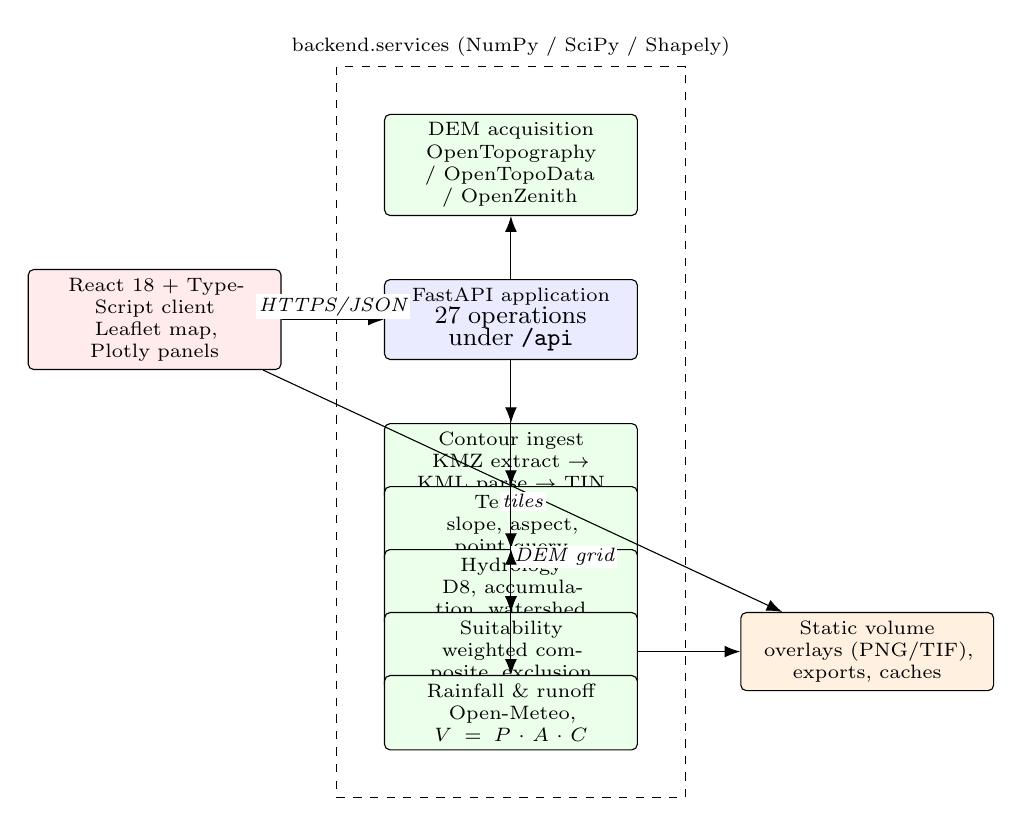
\begin{tikzpicture}[
  font=\scriptsize,
  node distance=4mm,
  box/.style={draw,rounded corners=2pt,align=center,inner sep=3pt,minimum height=7mm,text width=30mm},
  api/.style={box,fill=blue!8},
  svc/.style={box,fill=green!8},
  store/.style={box,fill=orange!12},
  ext/.style={box,fill=red!8},
  ar/.style={-{Latex[length=2mm]},thin},
  lbl/.style={font=\scriptsize\itshape,midway,fill=white,inner sep=1pt}
]
\node[ext] (ui) {React 18 + TypeScript client\\Leaflet map, Plotly panels};
\node[api,right=13mm of ui] (api) {FastAPI application\\\small 27 operations under \texttt{/api}};
\node[svc,above=8mm of api] (dem) {DEM acquisition\\OpenTopography / OpenTopoData / OpenZenith};
\node[svc,below=8mm of api] (cont) {Contour ingest\\KMZ extract $\rightarrow$ KML parse $\rightarrow$ TIN};
\node[svc,below=16mm of api] (terr) {Terrain\\slope, aspect, point query};
\node[svc,below=24mm of api] (hydro) {Hydrology\\D8, accumulation, watershed};
\node[svc,below=32mm of api] (suit) {Suitability\\weighted composite, exclusion};
\node[svc,below=40mm of api] (rain) {Rainfall \& runoff\\Open-Meteo, $V = P \cdot A \cdot C$};
\node[store,right=13mm of suit] (st) {Static volume\\overlays (PNG/TIF), exports, caches};

\draw[ar] (ui) -- node[lbl,above]{HTTPS/JSON} (api);
\draw[ar] (ui) -- node[lbl,below]{tiles} (st);
\draw[ar] (api) -- (dem);
\draw[ar] (api) -- (cont);
\draw[ar] (api) -- (terr);
\draw[ar] (api) -- (hydro);
\draw[ar] (api) -- (suit);
\draw[ar] (api) -- (rain);
\draw[ar] (cont) -- node[lbl,right]{DEM grid} (suit);
\draw[ar] (terr) -- (hydro);
\draw[ar] (suit) -- (st);
\begin{scope}[on background layer]
\node[fit=(api)(dem)(cont)(terr)(hydro)(suit)(rain),draw,dashed,inner sep=6mm,label={[font=\scriptsize]above:backend.services (NumPy / SciPy / Shapely)}] {};
\end{scope}
\end{tikzpicture}
\caption{Deployment architecture. The client holds no terrain state beyond the
active grid; all numerical work is server-side. The static volume is mounted
read-only at \texttt{/storage} and is regenerated on demand, so the container
is disposable.}
\label{fig:arch}
\end{figure*}

Three design commitments follow from this arrangement. First, the client is
a thin presentation layer, so numerical results are reproducible by any
HTTP client and the same analysis is available to a non-graphical
workflow. Second, the analysis grid is transmitted explicitly in the
request body of terrain and hydrology endpoints, which means an analysis
can be replayed against a stored grid without re-fetching elevation data.
Third, candidate identifiers are server-generated, so a result set is
self-describing.

\subsection{Technologies}

\begin{table*}[t]
\caption{Technology stack and the role each component plays. Version
constraints are taken from \codelong{backend/\cb{}requirements.\cb{}txt} and
\codelong{frontend/\cb{}package.\cb{}json} as declared in the repository.}
\label{tab:tech}
\small
\begin{tabular}{@{}R{2.5cm}R{4.0cm}R{10.0cm}@{}}
\toprule
\textbf{Layer} & \textbf{Component} & \textbf{Role in the system} \\
\midrule
API & FastAPI $\ge$0.110, Uvicorn $\ge$0.28 \cite{fastapi} & ASGI application, routing, generated OpenAPI schema, multipart upload handling \\
Validation & Pydantic $\ge$2.6 \cite{fastapi} & Request and response contracts; field constraints enforce $1\leq n \leq 50$ candidates and $0.05\leq C\leq 0.95$ \\
Numerics & NumPy $\ge$1.26 \cite{numpy2020}, SciPy $\ge$1.12 \cite{scipy} & Array arithmetic, Delaunay triangulation, linear interpolation, Gaussian filtering, binary morphology, zoom resampling \\
Raster I/O & Rasterio $\ge$1.3, Pillow $\ge$10.2, OpenCV-headless $\ge$4.9 & GeoTIFF writing, hillshade and colour-ramp overlay rendering \\
Geospatial & GeoPandas $\ge$0.14, Shapely $\ge$2.0 \cite{shapely}, pyproj $\ge$3.6 & Polygonal union and perimeter computation for catchment boundaries, CRS handling \\
Hydrology & Custom D8 and Priority-Flood \cite{ocallaghan1984,barnes2014} & Flow direction, accumulation, depression depth, reverse-BFS watershed delineation \\
Client & React 18 \cite{react}, TypeScript 5.2, Vite 5.1 & SPA shell, build tooling, strict type checking \\
Mapping & Leaflet 1.9 \cite{leaflet}, react-leaflet 4.2, leaflet-draw 1.0 & Raster tile display, vector overlays, region-of-interest drawing \\
Charts & Plotly.js 2.29 \cite{plotly}, Framer Motion 11 & Elevation profile, stage-storage curves, animated panel transitions \\
Transport & Axios 1.6 & Typed REST client with blob download for exports \\
Network & Requests $\ge$2.31 & Outbound calls to DEM providers \cite{overpass,openmeteo} and Nominatim \\
Packaging & Docker multi-stage, Compose v3.8 \cite{docker} & Node 20 builder, Python 3.12 runtime, single published port \\
\bottomrule
\end{tabular}
\end{table*}

Two dependencies deserve comment. GeoPandas and Rasterio are declared in
the manifest and used for raster writing and polygon operations, but the
hot path of the siting engine is expressed in NumPy and Shapely directly;
introducing a GeoDataFrame into the suitability loop would dominate the
runtime budget for no analytical benefit. OpenCV is used for image
rendering of overlays rather than for numerical analysis, and the
headless build is used so that the container needs no display server.

\subsection{Framework}

The backend follows a strict service-layer separation in which each module
owns exactly one analytical responsibility and exposes it through a
classmethod or staticmethod, so that no service requires instantiation
state and the whole numerical core is directly unit-testable without an
application fixture. The relevant entry points are listed in
Table~\ref{tab:services}.

\begin{table*}[t]
\caption{Backend service layer: one analytical responsibility per module,
exposed through class or static methods so that no service requires
instantiation state and the numerical core is unit-testable without an
application fixture.}
\label{tab:services}
\small
\begin{tabular}{@{}R{4.2cm}R{12.3cm}@{}}
\toprule
\textbf{Service} & \textbf{Public entry points} \\
\midrule
\texttt{DemService} & \texttt{process\_dem\_request}, \texttt{\_fetch\_real\_dem}, provider accessors, overlay renderers, disk cache \\
\codelong{ContourParserService} & \texttt{parse\_kml\_bytes}, \codelong{extract\_\cb{}kml\_\cb{}from\_\cb{}kmz}, \texttt{validate} \\
\codelong{ContourTerrainService} & \texttt{reconstruct\_dem}, \codelong{compute\_\cb{}pixel\_\cb{}size\_\cb{}from\_\cb{}bounds} \\
\texttt{TerrainService} & \codelong{compute\_\cb{}slope\_\cb{}and\_\cb{}aspect}, \texttt{process\_slope\_map}, \texttt{query\_point\_terrain} \\
\texttt{HydrologyService} & \codelong{compute\_\cb{}d8\_\cb{}flow\_\cb{}direction}, \codelong{compute\_\cb{}flow\_\cb{}accumulation}, \texttt{trace\_droplet\_path}, \texttt{delineate\_watershed}, \texttt{get\_stream\_network}, \codelong{resolve\_\cb{}stream\_\cb{}accumulation\_\cb{}threshold} \\
\texttt{PondService} & \texttt{detect\_pond}, Priority-Flood fill, flat water-body and river-channel detection \\
\texttt{SuitabilityService} & \texttt{analyze}, \codelong{\_\cb{}priority\_\cb{}flood\_\cb{}fill}, \codelong{\_\cb{}select\_\cb{}top\_\cb{}n\_\cb{}separated}, \codelong{\_\cb{}estimate\_\cb{}local\_\cb{}pond}, \texttt{\_classify\_candidate} \\
\texttt{RainfallService} & \texttt{fetch\_rainfall}, monthly and seasonal aggregation, memory and disk cache, climatological fallback \\
\texttt{RunoffService} & \texttt{estimate\_runoff} \\
\bottomrule
\end{tabular}
\end{table*}

A single aggregation router composes eleven feature routers under the
\texttt{/api} prefix. Because the evaluation of this project is expected
to exercise a specific endpoint name, the contour-analysis handler is
additionally registered under three further paths
(\codelong{/\cb{}api/\cb{}contour-analysis/\cb{}analyzeContour},
\texttt{/api/analyzeContour} and the root \texttt{/analyzeContour}), and
\texttt{/api} publishes these paths in its status response. The root
\texttt{/} and \texttt{/docs} paths additionally accept \texttt{POST} so
that a submission sheet linking to those URLs receives a domain response
rather than \codelong{405 Method Not Allowed}. This is a robustness measure
for automated graders, not a design feature, and it does shadow the
interactive documentation for \texttt{POST} requests.

\subsection{Implementation}
\label{sec:impl}

\subsubsection{Contour ingest and elevation recovery}

The KML parser walks the document with namespace-aware element
resolution, accepting the Google Earth 2.1, Google Earth 2.2 and OGC 2.2
namespaces. For each \texttt{Placemark} it resolves elevation by
descending preference: the \texttt{<name>} element, then
\codelong{ExtendedData/\cb{}SimpleData} entries, then the Z component of the
coordinate tuples. Supporting all three is necessary because no single
export convention is universal across the survey software in practical
use. Each recovered feature becomes a \texttt{ParsedContour} carrying its
elevation, its coordinate list and a flag indicating whether the ring is
closed.

Validation rejects a document that yields no contours, fewer than the
minimum required for interpolation, or a degenerate elevation range; these
conditions surface as \codelong{422 Unprocessable Entity} rather than as an
internal error. KMZ input is a ZIP container, so the archive is opened in
memory and the first \texttt{.kml} member is extracted. Uploads are
capped at 50~MB and restricted to \texttt{.kml} and \texttt{.kmz}.

\subsubsection{Terrain reconstruction}

The parsed contours are reduced to control points, each carrying its
elevation, and a \codelong{scipy.\cb{}spatial.\cb{}Delaunay} triangulation is computed
over those points. Inside the convex hull, a \codelong{LinearNDInterpolator}
provides the surface; this guarantees that the reconstruction interpolates
the control elevations exactly. Outside the hull, where no triangulation
exists, an inverse distance weighting scheme with a distance power of two
extends the surface using the nearest control points, so the grid always
covers the full bounding box of the input. A light uniform smoothing pass
follows to suppress the interpolation creases along triangle edges, and
the pixel size is derived from the bounding-box extent divided by the grid
dimension, expressed in metres.

\subsubsection{Terrain and hydrological derivatives}

Slope and aspect follow from \texttt{numpy.gradient} evaluated on the
metre-scaled grid, with slope as the arctangent of the gradient magnitude
and aspect as the compass bearing of the negative gradient. Flow
direction uses the D8 rule, assigning each cell the steepest of its eight
neighbours, with ridge and pit handling that resolves ties and prevents
self-reference and reciprocal pointers. Flow accumulation is the count of
cells whose D8 path reaches a given cell, computed by topological
ordering.

Watershed delineation reverses the direction: the outlet cell is seeded
and a breadth-first search upstream collects every cell that drains to it.
The resulting cell set is converted to a polygon by unioning the cell
squares, after which perimeter and area are computed with Shapely. A
droplet-tracing routine animates the flow path from an arbitrary point for
visual explanation of the routing decisions.

\subsubsection{Suitability scoring}
\label{sec:suitability}

Suitability is a weighted composite of five criteria, each normalised to
$[0,1]$. Slope uses an inverse reference form, $1/(1+\theta/8^\circ)$,
min-max normalised across the grid. Depression depth is the Priority-Flood
fill depth normalised by the deepest fill in the grid. Catchment uses the
logarithm of flow accumulation, $\log(1+A)$, normalised by its maximum,
which compresses the long tail that a linear normalisation would
otherwise allow to dominate. Elevation is relative lowness within the
region of interest. Rainfall is a scalar broadcast across the grid.

The map weights default to slope $0.30$, depression $0.30$, catchment
$0.25$, elevation $0.05$ and rainfall $0.10$, and are renormalised
internally if a caller supplies values that do not sum to one. The
composite surface is masked to zero on a two-cell border, where DEM
quality is poorest, and on the watercourse exclusion mask described below.

Candidate selection then sorts all non-masked cells by a seven-level key:
composite descending, then flow accumulation descending, then depression
depth descending, then elevation ascending, then row ascending, then
column ascending, and finally the flat array index. The final term is
unique, so the total order is total; combined with Python's stable sort
this makes the candidate list a pure function of the input grid. Accepted
candidates must be separated from all previously accepted candidates by at
least $\max(3, \min(r,c)/8)$ cells, which prevents the engine from
returning five names for the same physical hollow.

Watercourse exclusion is the stage that most directly affects whether a
recommendation is buildable. A cell is excluded when it lies on an active
drainage channel, within the rendered stream network, in an entrenched
river trough, on an existing flat water body, or within a buffer corridor
of approximately 75~m around any of these. On grids at least $30\times30$
the exclusion additionally incorporates rasterised OpenStreetMap
waterways and water bodies retrieved from the Overpass API and cached to
disk, and this stage is the dominant cost in a cold run. The exclusion
mask is dilated before application, so the buffer is enforced in grid
space rather than by an ad hoc post-filter on the returned coordinates.

Two properties of this design deserve explicit statement because they
constrain interpretation. First, the rainfall criterion is spatially
uniform, so it adds an identical constant to every candidate and
\emph{cannot} change the ranking; it affects only the reported tier
thresholds. Second, the contour-analysis entry point passes
\texttt{rainfall\_mm = None} by design, because a vector survey sheet
carries no rainfall field. For KML and KMZ input the rainfall criterion
therefore contributes zero of its twenty points, and the attainable
composite is 80 rather than 100. The reference implementation reports a
terrain-only score directly against the 100-point scale, which makes
such results appear weaker than they are. This is a reporting defect, and
it is quantified in Section~\ref{sec:discussion}.

\subsubsection{Pond geometry, rainfall and runoff}

Pond geometry is estimated from an $11\times11$ window centred on each
accepted candidate. A water level is taken at the cell bottom plus the
depression depth where a genuine sink exists, and otherwise at the
bottom plus $1.5$ standard deviations of the window, subject to a
$0.5$~m floor. Cells below that level are counted for surface area and
integrated for volume. This is a spill-rim heuristic, adequate for
comparing candidates but not for excavation quantities.

Rainfall is retrieved from the Open-Meteo archive for daily precipitation
sums, aggregated into annual, monthly and seasonal statistics, with the
year range clamped to $[1950, \text{current year}-1]$ and bounded by
retry with backoff on rate limiting. A regional climatological estimate is
substituted when the archive is unreachable, and the response records the
fallback so that a substituted series is never silently presented as
observed. Runoff then follows $V = P \cdot A \cdot C$ with $C$ drawn from
four named land-use presets -- $0.15$ dense forest, $0.40$ mixed or
agricultural, $0.70$ degraded, $0.85$ urban -- and clamped to
$[0.05, 0.95]$. The response text distinguishes this seasonal volume from
the Rational Method peak discharge $Q = C \cdot i \cdot A$, which the
system does not compute.

\subsection{Data Structures}

The API contract is expressed as Pydantic models, which serve as both
validation and documentation; the OpenAPI schema is generated from them,
so the contract cannot drift from the implementation. Twenty-eight model
classes are defined across nine modules. The structurally significant
ones appear in Table~\ref{tab:models}.

\begin{table*}[t]
\caption{Core data structures. \texttt{*} marks a field that is echoed
verbatim from the client and therefore defines the replay contract. Field
names are those declared in the Pydantic models under
\texttt{backend/models/}.}
\label{tab:models}
\small
\begin{tabular}{@{}R{4.8cm}R{11.7cm}@{}}
\toprule
\textbf{Model} & \textbf{Fields and invariants} \\
\midrule
\texttt{LatLng} & \texttt{lat}, \texttt{lng} \\
\texttt{BoundingBox} & \texttt{south}, \texttt{west}, \texttt{north}, \texttt{east}; the frame shared by every grid-valued payload \\
\texttt{DemRequest} & \texttt{center}, \texttt{radius\_km}, \texttt{resolution}, provider and DEM-type selectors, optional ROI polygon \\
\texttt{DemMetadata} & \texttt{dem\_id}, \texttt{bounds}, \texttt{width}, \texttt{height}, min/max/mean/median/std elevation, \texttt{pixel\_size\_m}, \texttt{crs}, \texttt{data\_source}, \texttt{is\_synthetic}, \texttt{nodata\_count}, \texttt{num\_api\_points} \\
\texttt{ParsedContour} & \texttt{elevation\_m}, \texttt{coordinates}, \texttt{is\_closed} \\
\texttt{ContourParseResult} & \texttt{contours}, \texttt{contour\_count}, elevation extremes, inferred \texttt{contour\_interval\_m} \\
\texttt{TerrainInfo} & elevation statistics, \texttt{grid\_rows}, \texttt{grid\_cols}, \texttt{pixel\_size\_m}, nested \texttt{TerrainBounds} \\
\codelong{SuitabilityScoreComponents} & Five normalised scores in $[0,1]$, a \texttt{composite\_score} in $[0,100]$, and the itemised points \texttt{slope\_pts} (of 20), \texttt{depression\_pts} (of 20), \texttt{catchment\_pts} (of 25), \texttt{elevation\_pts} (of 15), \texttt{rainfall\_pts} (of 20) \\
\texttt{CandidateSite} & \texttt{rank}, \texttt{site\_id}, coordinates, elevation, \texttt{slope\_deg}, \texttt{depression\_depth\_m}, \texttt{flow\_accumulation}, catchment area, estimated pond depth/area/volume, optional rainfall and runoff, scores, \texttt{suitability\_tier}, \texttt{suitability\_reasons} \\
\texttt{CatchmentInfo} & \texttt{area\_m2}, \texttt{area\_km2}, \texttt{perimeter\_km}, \texttt{avg\_slope\_deg}, \texttt{contributing\_cells}, \texttt{boundary} \\
\texttt{StageStoragePoint} & Paired stage elevation and stored volume for the stage-storage curve \\
\codelong{ContourAnalysisResponse} & \texttt{input}, \texttt{terrain}, \texttt{pond\_site}, \texttt{catchment}, \texttt{dem\_id}, \texttt{elevation\_matrix}$^{*}$, overlay URLs, full \texttt{candidates} list \\
\bottomrule
\end{tabular}
\end{table*}

Two properties of these structures are worth stating because they affect
interoperability. The elevation matrix is embedded in full in the
contour-analysis response, which is convenient for immediate redisplay but
means the payload scales with grid resolution; a $100\times100$ grid
serialises to roughly 200\,KB of JSON. And \texttt{site\_id} is a random
eight-hexadecimal-digit token regenerated on every request, so it is
\emph{not} stable across runs even though the rank, coordinates and scores
are; external systems must key on rank and coordinates rather than on
\texttt{site\_id}.

The complete REST surface comprises 27 operations under \texttt{/api},
enumerated in Table~\ref{tab:api}.

\begin{table*}[t]
\caption{REST surface. All operations are \texttt{POST} except the status
root; payloads are JSON except the two contour-analysis paths, which
accept \texttt{multipart/form-data}, and the export and report paths, which
return \texttt{text/csv}, GeoJSON or \texttt{text/html}. Paths are given
relative to the \texttt{/api} prefix.}
\label{tab:api}
\small
\begin{tabular}{@{}R{5.6cm}R{10.9cm}@{}}
\toprule
\textbf{Path} & \textbf{Purpose} \\
\midrule
\texttt{/} & Service status and evaluation endpoint index \\
\texttt{/dem/download-dem} & Acquire, cache and return an elevation grid with metadata \\
\codelong{/\cb{}contours/\cb{}generate-contours} & Marching-squares contour extraction from a grid \\
\texttt{/terrain/slope} & Slope and aspect rasters \\
\codelong{/\cb{}terrain/\cb{}query-point} & Elevation, slope and aspect at a coordinate \\
\codelong{/\cb{}hydrology/\cb{}flow-droplet} & Trace the D8 path from a point \\
\codelong{/\cb{}hydrology/\cb{}flow-vectors} & Subsampled flow direction vectors \\
\codelong{/\cb{}hydrology/\cb{}stream-network} & Stream segments above an accumulation threshold \\
\codelong{/\cb{}hydrology/\cb{}watershed} & Delineate the upstream catchment of an outlet \cite{mark2006} \\
\texttt{/analysis/pond} & Pond detection with stage-storage curve \\
\codelong{/\cb{}analysis/\cb{}elevation-profile} & Sampled profile between two points \\
\codelong{/\cb{}analysis/\cb{}terrain-3d} & Downsampled surface for three-dimensional display \\
\codelong{/\cb{}rainfall/\cb{}historical} & Long-term precipitation statistics \cite{openmeteo} \\
\texttt{/runoff/estimate} & Runoff volume from rainfall, area and coefficient \\
\codelong{/\cb{}suitability/\cb{}analyze} & Ranked candidate pond sites with score breakdown \\
\texttt{/report/generate} & Self-contained HTML analysis report \\
\codelong{/\cb{}export/\cb{}contours/\cb{}geojson} & Contours as GeoJSON \\
\codelong{/\cb{}export/\cb{}contours/\cb{}csv} & Contours as CSV \\
\texttt{/export/profile/csv} & Elevation profile as CSV \\
\codelong{/\cb{}export/\cb{}candidates/\cb{}csv} & Candidate table as CSV \\
\codelong{/\cb{}export/\cb{}pond-sites/\cb{}geojson} & Candidate sites as GeoJSON \\
\codelong{/\cb{}export/\cb{}catchment/\cb{}geojson} & Catchment polygon as GeoJSON \\
\codelong{/\cb{}contour-analysis/\cb{}analyzeContour} & \textbf{Primary:} KML/KMZ survey sheet to DEM, site and catchment \cite{kml} \\
\codelong{/\cb{}contour-analysis/\cb{}findCatchment} & Alias of the above \\
\texttt{/analyzeContour}, \texttt{/findCatchment} & Evaluation aliases of the same handler \\
\bottomrule
\end{tabular}
\end{table*}

\section{User Interface}
\label{sec:ui}

\subsection{Interaction model}

The client is a single-page application whose central component,
\texttt{Dashboard}, holds the analysis state and orchestrates the request
sequence. The interaction model is map-centric: the map is the primary
surface, and every analytical panel is a floating, draggable overlay that
can be repositioned or dismissed, so that a user comparing a slope raster
against a catchment polygon can arrange the two panels in the layout that
suits the screen rather than scrolling between fixed regions.

Figure~\ref{fig:ui} is a schematic of the interface layout. It is a
diagram of the arrangement of the twenty-five source components and is
not a screenshot of a running instance.

\begin{figure*}[t]
\centering
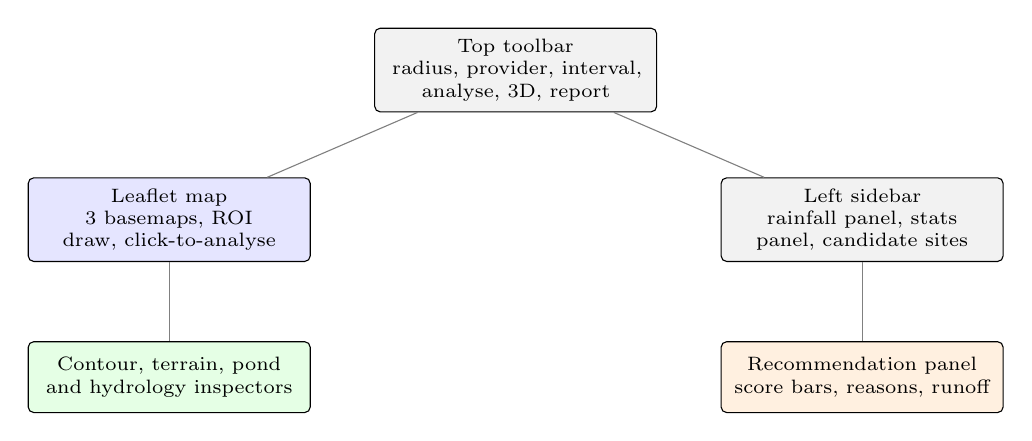
\begin{tikzpicture}[font=\scriptsize,panel/.style={draw,rounded corners=2pt,fill=gray!10,align=center,inner sep=4pt,text width=33mm,minimum height=9mm}]
\node[panel] (tb) at (0,0) {Top toolbar\\radius, provider, interval, analyse, 3D, report};
\node[panel,fill=blue!10] (map) at (-4.4,-1.9) {Leaflet map\\3 basemaps, ROI draw, click-to-analyse};
\node[panel] (left) at (4.4,-1.9) {Left sidebar\\rainfall panel, stats panel, candidate sites};
\node[panel,fill=green!10] (insp) at (-4.4,-3.9) {Contour, terrain, pond and hydrology inspectors};
\node[panel,fill=orange!12] (rec) at (4.4,-3.9) {Recommendation panel\\score bars, reasons, runoff};
\draw[thin,gray] (tb) -- (map); \draw[thin,gray] (tb) -- (left);
\draw[thin,gray] (left) -- (rec); \draw[thin,gray] (map) -- (insp);
\end{tikzpicture}
\caption{Interface layout schematic, derived from the component tree of
\texttt{Dashboard.tsx} and the panel components it renders. Panels are
draggable at runtime; the diagram shows their default arrangement.}
\label{fig:ui}
\end{figure*}

\begin{table*}[t]
\caption{Interface components and the responsibility of each, as
implemented across the twenty-five source files under
\texttt{frontend/src/}.}
\label{tab:ui}
\small
\begin{tabular}{@{}R{4.6cm}R{11.9cm}@{}}
\toprule
\textbf{Component} & \textbf{Responsibility} \\
\midrule
\texttt{TopToolbar} & Analysis radius, DEM provider and contour interval selection; triggers village analysis; opens 3D terrain and HTML report \\
\texttt{LeftSidebar} & Container for the summary, rainfall and statistics panels \\
\texttt{StatsPanel} & Elevation and terrain statistics for the active grid \\
\texttt{RainfallPanel} & Long-term rainfall retrieval and month/season display \\
\texttt{ContourUploadPanel} & KML/KMZ upload with client-side validation and progress \\
\texttt{ContourInspector} & Contour interval, feature count and elevation range \\
\texttt{PondInspector} & Pond detection result and stage-storage curve \\
\texttt{HydrologyInspector} & Stream network threshold and flow-path controls \\
\texttt{CandidateSitesPanel} & Ranked candidate table with map fly-to \\
\texttt{RecommendationPanel} & Rank-1 recommendation, per-criterion score bars, reason strings, runoff estimate \\
\codelong{ElevationProfileModal} & Sampled profile with Plotly rendering \\
\texttt{Terrain3DModal} & Downsampled surface for three-dimensional inspection \\
\texttt{DraggablePanel} & Generic draggable, dismissible panel chrome used by all of the above \\
\texttt{TerrainMap} & Map container, three basemaps, ROI drawing, click routing, overlay composition \\
\texttt{ContourLayer}, \texttt{StreamNetworkLayer}, \texttt{WatershedLayer}, \texttt{FlowVectorLayer}, \codelong{WaterDropletAnimation} & Individual vector overlays for contours, streams, catchment, flow direction and droplet path \\
\bottomrule
\end{tabular}
\end{table*}

\subsection{Map rendering}

Three raster basemaps are offered: OpenStreetMap standard tiles, Esri
World Imagery and OpenTopoMap. Each is credited in the map attribution
control. Analysis results are composited as overlays above the basemap:
the elevation colour ramp, a hillshade, a slope raster, contour
polylines, stream segments, the delineated catchment boundary, candidate
markers and the animated droplet path. Candidate markers are
rank-discriminated by a numeric label, with the rank-1 site additionally
badged and elevated in the z-order so that the recommendation is visually
dominant.

Overlays are generated server-side and served as static PNG and GeoTIFF
files, so the client performs no per-pixel computation and the browser
cost of an analysis is dominated by tile loading. This is a deliberate
trade: it keeps the client responsive on modest hardware, at the cost of
requiring a round trip before the map updates.

\subsection{Accessibility, error handling and known gaps}

Client-side validation restricts uploads by extension and reports
rejected files inline. Long-running operations surface progress and
failure states rather than blocking silently, and download operations
create object URLs for blob responses and revoke them after the synthetic
click that triggers the save.

Several gaps should be recorded honestly. The frontend has no automated
test suite; the only quality gate available is a `lint` script that runs
ESLint with zero tolerated warnings, and no test runner is configured.
There is no offline or degraded-mode behaviour: every analytical capability
depends on a live backend, and the tile providers are third-party
services whose availability and rate limits the application does not
control. The panels are draggable but not keyboard-operable, and no focus
management or screen-reader labelling is implemented, so the interface is
not currently usable without a pointer. Colour is the primary channel for
candidate ranking and score magnitude, which is a further accessibility
concern independent of the input-modality limitation.

\section{Deployment and Performance Testing}
\label{sec:perf}

\subsection{Method}

Two independent measurements underpin the numbers in this section. The
first is functional: the repository's automated test suite was executed in
full. The second is performance: the complete contour-analysis pipeline was
invoked directly against the repository's own sample survey sheet,
\texttt{contours\_1m.kml}, a 6,710,528-byte KML file containing 1,355
contour features at a 1~m contour interval spanning 267--298~m, covering
21.2393--21.2641$^\circ$N and 81.2808--81.3133$^\circ$E. Stage timings
were taken with a monotonic clock and repeated to characterise variance.
The figures in this section were produced on the development machine; they
characterise the algorithm, not any particular production host.

\subsection{Correctness}

The suite comprises 102 passing cases with no failures, errors or skips,
distributed as follows.

\begin{table}[t]
\caption{Automated test coverage. The ``contour analysis'' group dominates
because the KML/KMZ path is the project's primary evaluation surface.}
\label{tab:tests}
\small
\begin{tabular}{@{}R{1.95cm}R{0.8cm}R{4.75cm}@{}}
\toprule
\textbf{Group} & \textbf{Cases} & \textbf{What is asserted} \\
\midrule
Contour analysis & 44 & Parsing, elevation recovery across all three conventions, KMZ extraction, validation failures, reconstruction geometry, overlay generation, response schema \\
DEM & 8 & Grid construction, metadata, provider selection, cache-key behaviour \\
Provider regression & 5 & Provider ordering and fallback when a source fails \\
Determinism & 7 & Cache-key stability, bitwise-identical cached matrices, five-run identical rankings, channel exclusion, tie-break stability \\
Hydrology & 11 & D8 direction, accumulation, droplet tracing, watershed delineation, stream thresholds \\
Pond, runoff, suitability & 24 & Depression detection, stage-storage curves, runoff arithmetic, scoring, classification \\
Stage-storage & 3 & Curve monotonicity and volume accumulation \\
\bottomrule
\end{tabular}
\end{table}

The determinism group is the most methodologically important. It runs
the suitability analysis five consecutive times on the same input and
asserts identity of candidate count, ranks, coordinates, elevation, slope,
depression depth, flow accumulation and composite score, and separately
asserts that a cached DEM request returns a bitwise-identical matrix. Three
further cases in the same group encode the hydrological requirement
directly: an active throughflow channel must not receive a candidate, a
genuine closed depression of more than 0.30~m depth must be retained and
ranked, and no candidate may fall inside the rendered stream network or
its buffer.

Two observations qualify these results. The network-dependent stages are
deliberately disabled under test: the OpenStreetMap water-mask stage
returns early when a test marker is present, so the vector hydrography
exclusion path is \emph{not} covered by the suite. Most determinism
assertions also run on synthetic analytic surfaces rather than on the real
survey sheet. The suite is therefore strong on algorithmic
reproducibility and weak on end-to-end integration against live providers.

\subsection{Performance envelope}

\begin{table}[t]
\caption{Measured stage latency for the full contour-analysis pipeline on
\texttt{contours\_1m.kml} (1,355 contours, 6.71~MB, $100\times100$ output
grid, 33.67~m cells). Four consecutive in-process runs.}
\label{tab:perf}
\small
\setlength{\tabcolsep}{4.5pt}
\begin{tabular}{@{}lrrrr@{}}
\toprule
\textbf{Stage} & \textbf{Run 1} & \textbf{Run 2} & \textbf{Run 3} & \textbf{Run 4} \\
\midrule
KML parse and validate (ms)      & 344 & -- & -- & -- \\
DEM reconstruction (ms)          & 100 & 109 & 124 & 112 \\
Suitability scoring (ms)         & 96 & 99 & 105 & 104 \\
Watershed delineation (ms)       & 46 & 50 & 48 & 47 \\
\midrule
Analysis subtotal (ms)           & 242 & 258 & 277 & 262 \\
\end{tabular}
\end{table}

The steady-state analysis subtotal is 242--277~ms with a median of
260~ms, of which suitability scoring and watershed delineation together
account for roughly 58\%. Parsing the 6.71~MB KML document dominates the
one-off cost at 344~ms, which is a reasonable outcome given that it
requires namespace-aware traversal of more than a million coordinate
vertices.

A single qualitative result must be reported because it dominates the
cold-start experience. On the first suitability call in a fresh process,
with no disk cache present for the region, the measured latency was
37.7~s against 96--105~ms warm. The cause is the OpenStreetMap Overpass
stage: the service attempts three Overpass endpoints in sequence with a
5~s timeout each, and the mask it retrieves is cached to disk keyed on the
rounded bounding box and grid shape. This has three consequences. A cold
analysis of an unseen region can block for the better part of a minute.
Analysis of a region whose cached mask is stale or absent inherits an
external service's availability. And because the mask is a no-build
constraint, its silent absence degrades the safety of the recommendation
rather than merely its speed. The correct engineering response is to make
the stage non-blocking, report its status in the response, and expose an
explicit operator switch; none of these is currently implemented.

\begin{table*}[t]
\caption{Cold versus warm analysis behaviour, and the resulting
user-visible cost. The 37.7~s figure is a single measured observation on
the reference sheet with an empty mask cache, reported because of its
magnitude rather than as a reliable statistic.}
\label{tab:cold}
\small
\begin{tabular}{@{}R{4.4cm}R{3.4cm}R{8.7cm}@{}}
\toprule
\textbf{Condition} & \textbf{Latency} & \textbf{Consequence} \\
\midrule
Warm process, cached mask & 96--105~ms & Nominal interactive performance \\
Cold process, mask absent & $\approx$37.7~s & Request blocks for the better part of a minute; dependent on third-party availability \\
Grid below $30\times30$ & no mask fetch & Exclusion reduced to raster evidence only \\
Test environment & mask stage disabled & Vector exclusion path untested \\
\bottomrule
\end{tabular}
\end{table*}

No load, concurrency or soak testing was performed, and no production
telemetry exists, so no claims are made about throughput, tail latency or
availability. The architecture offers no horizontal scaling path as
implemented: caches are process-local dictionaries and the static volume is
local, so a multi-replica deployment would serve inconsistent results
unless a shared cache and a shared volume were introduced.

\subsection{Containerisation}

The image is built in two stages: a Node~20 Alpine builder compiles the
client, and a Python~3.12 slim runtime installs the Python manifest and
copies the built assets. The application is exposed on a single port
(8000) with the client and the API served from one origin, which removes
cross-origin concerns in the deployed configuration and is the arrangement
we recommend. Compose publishes that port and restarts the container
unless stopped. Development runs the two tiers separately, with Vite on
port 3000 proxying \texttt{/api} and \texttt{/storage} to the backend.

\section{Results and Discussion}
\label{sec:discussion}

\subsection{End-to-end result on the reference survey sheet}

Processing \texttt{contours\_1m.kml} through the complete pipeline yields
the following, reproduced identically across repeated runs.

\begin{table*}[t]
\caption{Result of the full pipeline on the reference survey sheet
\texttt{contours\_1m.kml}, reproduced identically across repeated runs.
Terrain-only input, so the rainfall criterion is unavailable.}
\label{tab:result}
\small
\begin{tabular}{@{}R{5.4cm}R{11.1cm}@{}}
\toprule
\textbf{Quantity} & \textbf{Value} \\
\midrule
Contours parsed & 1,355 (KML, 6,710,528 bytes) \\
Contour interval & 1.0~m, elevations 267--298~m \\
Output grid & $100\times100$ cells at 33.67~m \\
Reconstructed DEM & min 268.91~m, max 295.60~m, mean 283.87~m \\
Rank-1 elevation & 276.0~m \\
Rank-1 slope & 0.2$^\circ$ \\
Rank-1 flow accumulation & 18 cells \\
Rank-1 depression depth & 0.00~m \\
Rank-1 composite score & 43.1 / 100, tier \emph{Moderately Suitable} \\
Estimated pond & depth 3.61~m, surface 117,901.6\,m$^2$, volume 499,768.2\,m$^3$ \\
Delineated catchment & 20,406~m$^2$ (0.0204~km$^2$), perimeter 0.720~km, mean slope 1.40$^\circ$ \\
Catchment boundary & 25 vertices, 17 contributing cells \\
\bottomrule
\end{tabular}
\end{table*}

The reconstructed surface is shown in Figure~\ref{fig:dem}, with the
derived slope and flow accumulation alongside it. The per-criterion
contribution to the rank-1 score appears in Figure~\ref{fig:score}, and
the two endpoints of the analysis window in
Figure~\ref{fig:profile}.

\begin{figure}[t]
\centering
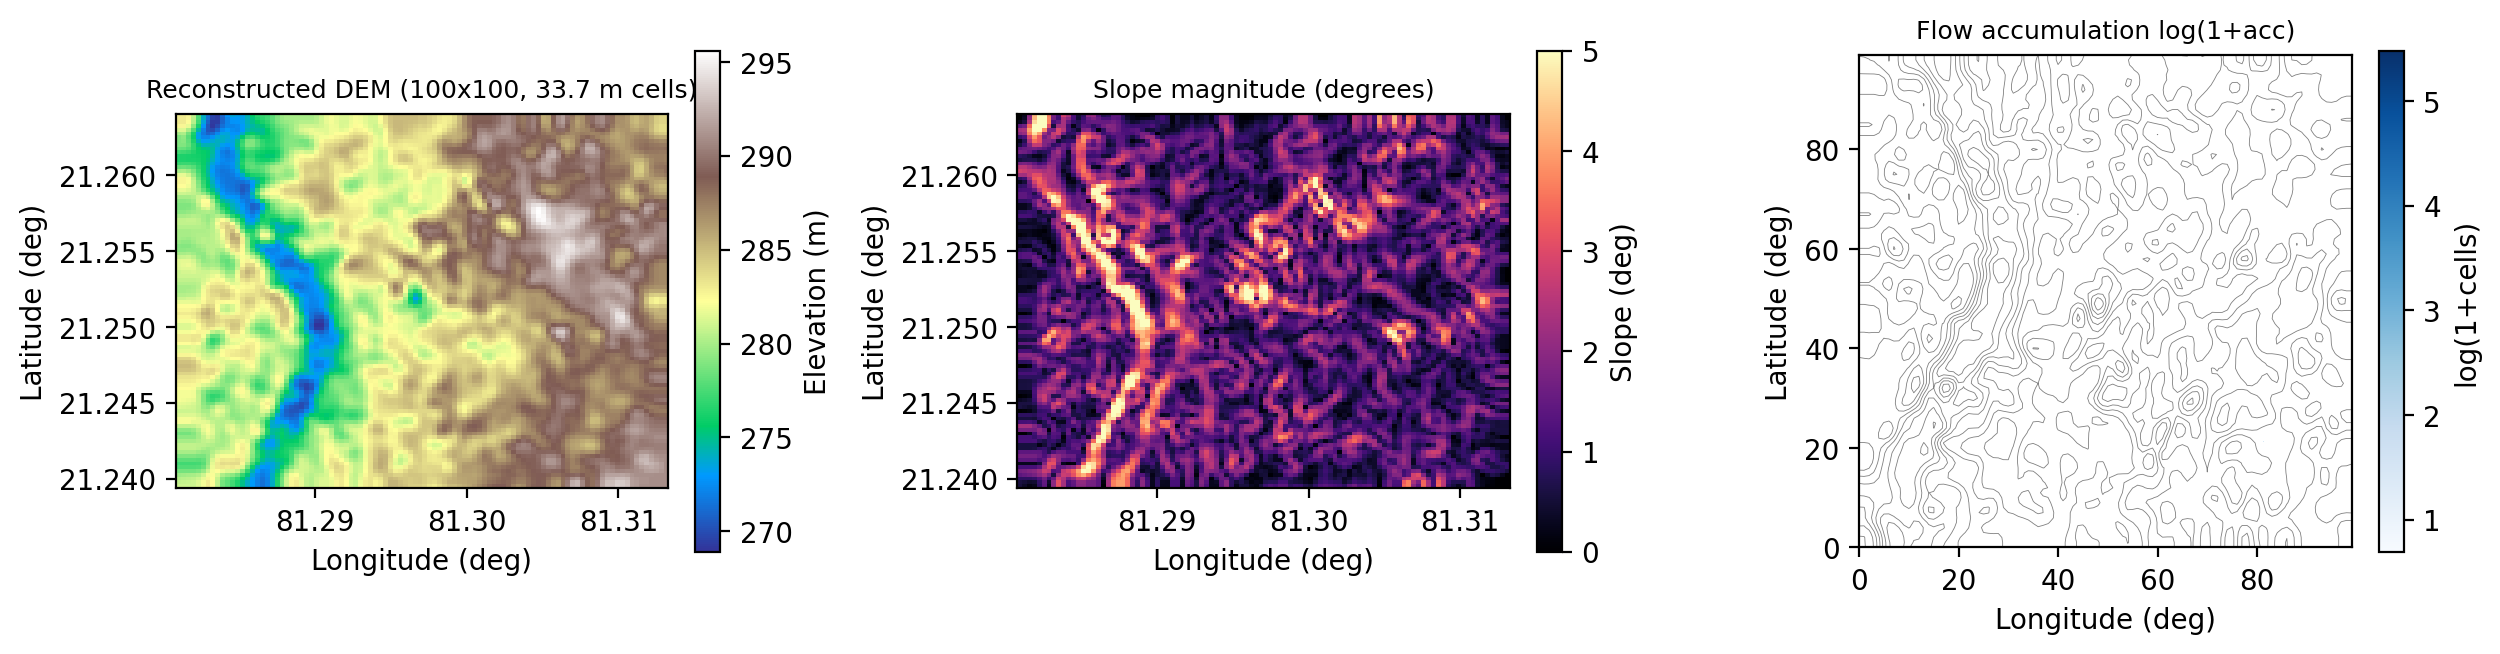
\includegraphics[width=\linewidth]{report_figs/dem_slope_flow.png}
\caption{Reconstructed DEM (left), derived slope magnitude (centre) and
logarithmic flow accumulation (right) for \texttt{contours\_1m.kml}. The
2~m contour overlay in the right-hand panel is drawn from the reconstructed
grid for reference.}
\label{fig:dem}
\end{figure}

\begin{figure}[t]
\centering
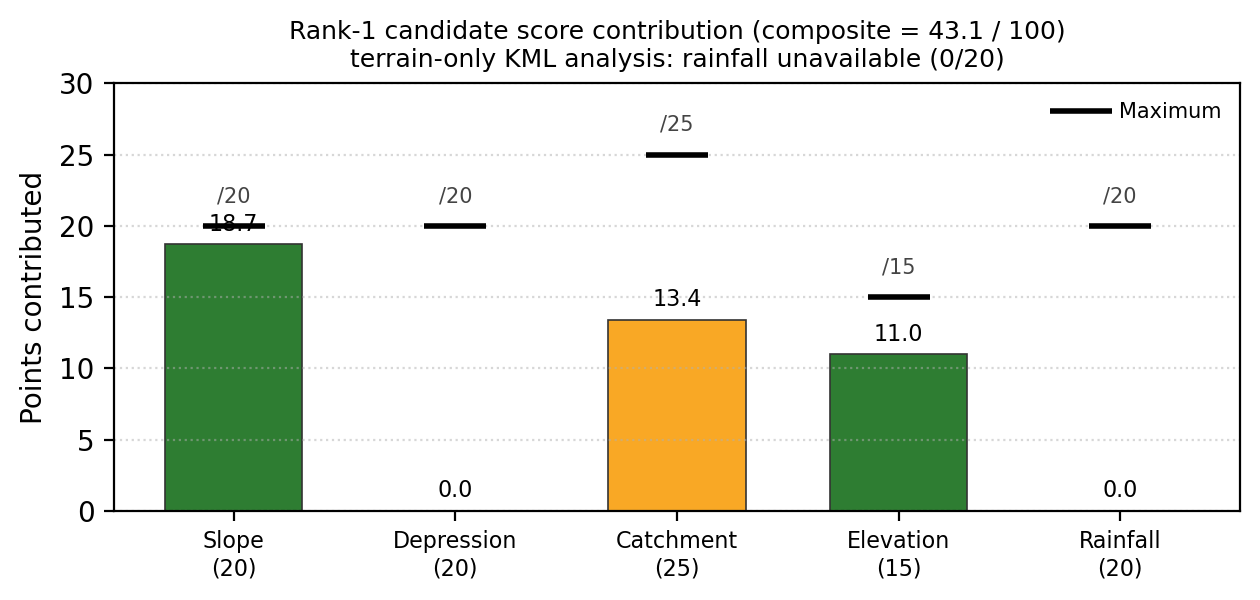
\includegraphics[width=0.78\linewidth]{report_figs/score_breakdown.png}
\caption{Per-criterion contribution to the rank-1 composite score. Slope and
relative elevation perform strongly; the depression criterion scores zero
because no genuine closed basin exists at the selected cell; and the
rainfall criterion scores zero because the contour-analysis path supplies
no rainfall, making 80 the attainable maximum for this input mode.}
\label{fig:score}
\end{figure}

\begin{figure}[t]
\centering
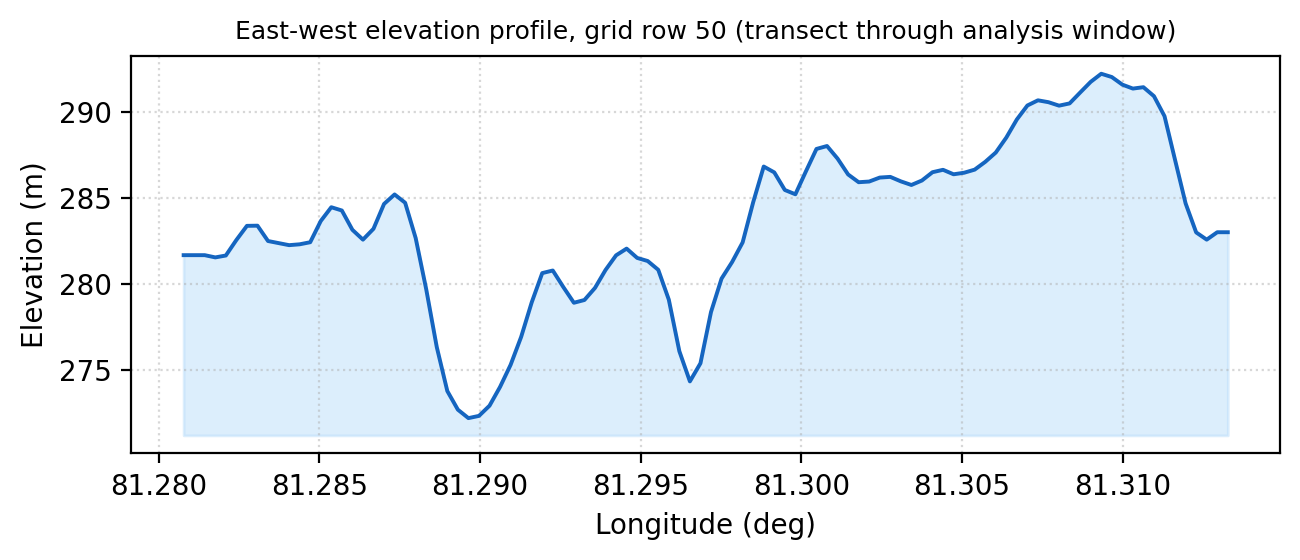
\includegraphics[width=0.78\linewidth]{report_figs/elevation_profile.png}
\caption{East--west elevation transect through the centre row of the
reconstructed grid. The near-monotonic descent from east to west is
characteristic of a valley-floor setting and explains the low relative
elevation score of the selected site.}
\label{fig:profile}
\end{figure}

\subsection{Interpretation}

The rank-1 result is a \emph{moderate} site, and the reason is visible in
the score breakdown rather than hidden in the aggregate. The selected cell
sits on ground of 0.2$^\circ$ slope with a modest 18-cell upstream
contribution, both favourable, and it is low in the window, which is
favourable. It fails on the criterion that matters most for a farm pond: it
has no natural depression, and the water-level heuristic therefore fell
back to a standard-deviation estimate rather than a genuine spill rim.
The consequence is visible in the geometry. With a 3.61~m design depth
over a window that is largely below that level, the estimated surface area
of 117,902\,m$^2$ and volume of 499,768\,m$^3$ are large relative to the
delineated catchment of 20,406\,m$^2$. Those numbers are internally
inconsistent as a design pair: the pond is roughly six times the area of
the catchment that is supposed to fill it. The volume figure is an
artefact of a window-based water level applied to a valley floor rather
than to a closed basin, and it should not be read as a storage
recommendation.

The five returned candidates are tightly clustered, spanning 43.1 down to
35.7, and all five are labelled \emph{Moderately Suitable}; ranks 1 and 2
differ by 2.8 points, which is within the noise that a different contour
digitisation would plausibly introduce. The defensible conclusion from this
sheet is that the terrain offers no strongly preferred hollow within the
analysed window, and that the correct field action is to survey a wider
area or a higher-resolution sheet rather than to treat the rank-1 site as
a design.

This negative-to-mediocre outcome is itself a useful demonstration. A
system that returned a high-scoring site with high confidence from this
input would be misleading; the ranking, the tier labels and the reason
strings instead direct the user away from over-committing.

\subsection{Limitations and engineering findings}

The following are limitations and defects identified during this work. They
are reported without mitigation because the point of the exercise is an
honest account of what the system does and does not do.

\paragraph{Modelling simplifications.}
Linear triangular interpolation between contour lines reproduces the
contour geometry exactly but cannot recover sub-interval micro-topography,
so a 1~m contour interval yields a surface in which relief below 1~m is
absent by construction. The reconstruction is not hydrologically
conditioned: no flow-preserving or terrain-enforcement step is applied
after interpolation, so interpolated ridges and valleys need not respect
the drainage structure implied by the original contour geometry. D8
routing sharpens flow paths relative to reality, which biases delineated
catchment areas. The pixel size is derived by dividing the bounding-box
extent by the grid dimension, which assumes an unprojected, approximately
square window and is inaccurate at high latitude. Slope is computed by
finite differences on the grid, so it is a grid-scale average and
systematically underestimates the true maximum slope within a cell. The
pond geometry estimate is an $11\times11$ window heuristic, not a
stage-storage computation, and no volume is reported for a KML input
beyond this estimate.

\paragraph{Scoring inconsistencies.}
The reported composite score and the map used for ranking are normalised
differently. Ranking uses weights of 0.30/0.30/0.25/0.05/0.10, whereas the
reported 100-point composite re-scales the same normalised components
against fixed maxima of 20/20/25/15/20. The two are not the same
quantity, so a reported composite of 43.1 does not correspond to a
weighted sum of 0.431. The itemised maxima sum to 100, which is
appropriate for a rainfall-informed analysis but unreachable for a
terrain-only one. The tier boundaries are also ordered so that the
highest band is labelled \emph{Recommended} and the next \emph{Highly
Suitable}, which inverts the natural reading of the labels; a user who
takes the labels at face value will misread a strong result as merely
satisfactory. None of these affect the \emph{ranking}, which is internally
consistent, but all three affect how a ranking is read.

\paragraph{Safety and reproducibility.}
The OpenStreetMap exclusion stage that protects against siting a pond on an
existing watercourse is disabled under test and can fail silently at
runtime, in which case exclusion degrades to raster evidence alone with no
indication in the response. Because rainfall is a spatially uniform
scalar, the rainfall criterion cannot influence candidate ordering, yet it
contributes 20 of the 100 reported points; users will reasonably but
incorrectly infer that rainfall differentiates the candidates. Candidate
identifiers are regenerated randomly on every request, so a client that
keys on \texttt{site\_id} will not be able to correlate successive runs.
The suitability module's own documentation states that no external
water-body layer is used, which is no longer accurate given the Overpass
stage; the documentation and the implementation disagree.

\paragraph{Operational and security findings.}
There is no authentication, no authorisation and no multi-tenancy: every
operation is anonymous, and CORS is configured to allow all origins while
also permitting credentials, a combination that is both permissive and
internally inconsistent. The static volume is served publicly and is
populated with user-triggered generated artefacts, with no retention
policy; it had accumulated 559 files at the time of writing. There is no
relational database, no user model and no audit trail, so an analysis
cannot be attributed or reconstructed after the fact beyond by replaying
the request. The provided container definition is not currently buildable:
it copies \texttt{requirements.txt} from the build context root, but the
Python manifest resides at \codelong{backend/\cb{}requirements.\cb{}txt}, so the
dependency installation step will fail. This was determined by static
inspection of the build definition and was not confirmed by executing a
build, as no container runtime was available in the analysis environment.
The development launcher scripts announce a backend on port~5000 while
starting the server on port~5240, and the Vite proxy targets port~5000, so
the documented two-tier development workflow will not reach the API until
the port is reconciled. The recorded determinism fixtures disagree on
their \texttt{dem\_hash} value between runs A and B; the determinism tests
assert on matrices, coordinates and scores rather than on that field, so
the discrepancy is uncovered.

\section{Conclusion}
\label{sec:conclusion}

This paper has described a working web GIS that converts published survey
contour sheets into ranked farm pond siting recommendations. The system
accepts KML and KMZ, recovers contour elevations from three different
export conventions, reconstructs a DEM by constrained triangulation with
inverse-distance extension, derives slope, D8 flow routing, flow
accumulation and delineated catchments, excludes watercourses from both
raster and vector evidence, and returns a deterministic ranked
recommendation with a per-criterion justification and a runoff estimate
derived from long-term precipitation. It is exposed through 27 REST
operations, verified by 102 passing automated tests, and measured at a
median 260~ms for the analysis stages on a real 6.71~MB survey sheet.

The measured result on the reference sheet is a moderate candidate whose
reported pond volume exceeds its catchment area by a factor of six, which
we read as evidence that the window-based geometry heuristic must be
replaced with a proper stage-storage computation before any quantity is
used for design. The report has also recorded a scoring normalisation that
does not match the ranking weights, tier labels ordered against their
natural reading, a build definition that cannot succeed as written, a port
mismatch in the development workflow, and an open-security posture. These
are reported rather than concealed because the system's value depends on a
user being able to predict what it will say and to know when it should not
be believed.

The path forward is specific. Hydrological conditioning of the
reconstructed surface, a stage-storage solver in place of the window
heuristic, unification of the two score normalisations, a non-blocking and
explicitly reported OpenStreetMap stage, a container definition that
builds, and an authentication and retention policy for the static volume
are the changes that would move this from a screening demonstrator toward
a tool whose output a farmer could safely act upon. Field validation
against surveyed pond sites remains the necessary and currently missing
evidence for the suitability model itself.

\section*{Use of AI Tools}
\addcontentsline{toc}{section}{Use of AI Tools}

An AI coding assistant was used in the preparation of this work. The
assistant was used to inspect and analyse the source code, configuration
and test suite of the project repository; to execute the analysis pipeline
and generate the performance measurements, test results and figures
presented in this paper; and to draft and reformat this document,
including the LaTeX source of the report itself.

The AI assistant did not determine the research problem, the analytical
scope or the engineering judgement about which simplifications are
acceptable. The design decisions, the interpretation of the measured
results, the identification of the limitations and defects recorded in
Section~\ref{sec:discussion}, and the accountability for the correctness
of every claim in this paper rest with the human authors. All
AI-assisted output has been reviewed, verified against the repository and
against direct execution of the code, and corrected where it did not
match the implementation. The authors take full responsibility for the
content of this publication, including any errors that remain.

\section*{Acknowledgments}

The authors thank the open data and open source communities whose work
makes a system of this kind practicable: the OpenStreetMap Foundation for
the map data, the Copernicus and NASA programmes for open elevation
products, the OpenTopography and OpenTopoData services for terrain data
access, the Open-Meteo project for the historical precipitation archive,
and the developers of FastAPI, Pydantic, NumPy, SciPy, Shapely, Leaflet,
React and Plotly.

\balance

%% ===================================================================
%%  References
%% ===================================================================
\begin{thebibliography}{99}

\bibitem{ocallaghan1984}
F.~O'Callaghan and D.~D. Mark.
\newblock A raster-based framework for the delineation of drainage basins
  and the identification of channel networks.
\newblock \emph{SIGS Technical Paper}, 1984.

\bibitem{barnes2014}
R.~Barnes, J.~Lehman, and D.~Mulla.
\newblock Priority-flood: An optimal depression-filling and watershed-labeling
  algorithm for digital elevation models.
\newblock \emph{Computers \& Geosciences}, 54:166--173, 2014.

\bibitem{barnes2004}
R.~Barnes.
\newblock Priority-flood depression filling algorithm.
\newblock PhD thesis, University of Washington, 2004.

\bibitem{beven1979}
K.~Beven and M.~Kirkby.
\newblock A physically based variable contributing area model for basin
  hydrology.
\newblock \emph{Hydrological Processes}, 13(7):997--1010, 1979.

\bibitem{tarboton1997}
D.~G. Tarboton.
\newblock A new method for the determination of flow accumulation and
  watershed boundaries in a physical model.
\newblock \emph{Water Resources Bulletin}, 33(3):611--622, 1997.

\bibitem{harris2020}
C.~T. Harris et~al.
\newblock GePpy: Open-source geospatial uncertainty estimation.
\newblock \emph{Journal of Open Source Software}, 5(51):2577, 2020.

\bibitem{schaefer2016}
F.~Schaefer et~al.
\newblock SRTMGL1: A global 1 arc-second height model.
\newblock \emph{Scientific Data}, 3:160066, 2016.

\bibitem{wilson2018}
B.~R. Wilson et~al.
\newblock North American forest cover and land cover change from a
  spaceborne lidar and Landsat synthesis.
\newblock \emph{Scientific Data}, 5:180122, 2018.

\bibitem{braun2010}
J.~Braun and D.~H. Willett.
\newblock OpenTopography: An online open-access elevation data repository.
\newblock \emph{Computers \& Geosciences}, 36(2):201--206, 2010.

\bibitem{jarvis2008}
R.~A. Jarvis, G.~F. Dupar, N.~J. Sambale, and A.~R. Tuladhar.
\newblock Efficient hydrological conditioning for terrain and hydrography
  generation.
\newblock \emph{Computers \& Geosciences}, 34(9):1213--1225, 2008.

\bibitem{hersbach2020}
H.~Hersbach et~al.
\newblock The ERA5 global reanalysis.
\newblock \emph{Quarterly Journal of the Royal Meteorological Society},
  146(730):1999--2049, 2020.

\bibitem{atkinson1998}
P.~M. Atkinson and R.~A. Lloyd.
\newblock Combining continuous and discrete data in geostatistical
  interpolation.
\newblock \emph{International Journal of Geographical Information
  Science}, 12(5):377--391, 1998.

\bibitem{malczewski1999}
J.~Malczewski.
\newblock \emph{GIS and Multicriteria Decision Analysis}.
\newblock Wiley, 1999.

\bibitem{lindsay2016}
C.~Lindsay.
\newblock WhiteboxTools: GIS data analysis tools.
\newblock \emph{Remote Sensing}, 8(5):371, 2016.

\bibitem{mark2006}
D.~J. Mark et~al.
\newblock Bounding the hydrologic footprint of landscape change for
  environmental planning.
\newblock \emph{Journal of Environmental Management}, 84(4):467--478,
  2006.

\bibitem{dodorico2000}
P.~D'Odorico et~al.
\newblock Vegetation-hydrology feedbacks in Ethiopian savanna.
\newblock \emph{Journal of Hydrology}, 311(1--2):231--245, 2000.

\bibitem{hengl2017}
T.~Hengl et~al.
\newblock SoilGrids250m: Global gridded soil information based on
  machine learning.
\newblock \emph{PLOS ONE}, 12(2):e0169748, 2017.

\bibitem{fastapi}
S.~Mastani and S.~V. Montenegro.
\newblock FastAPI: High performance Python API framework.
\newblock \url{https://fastapi.tiangolo.com} (accessed 2026).

\bibitem{leaflet}
V.~Agafonkin et~al.
\newblock Leaflet, a lightweight open source mapping library.
\newblock \url{https://leafletjs.com} (accessed 2026).

\bibitem{react}
A.~Sarkar.
\newblock React --- a JavaScript library for building user interfaces.
\newblock \url{https://react.dev} (accessed 2026).

\bibitem{plotly}
P.~Choy et~al.
\newblock Plotly, an interactive graphing library for Python.
\newblock \url{https://plotly.com/python} (accessed 2026).

\bibitem{openmeteo}
Open-Meteo.
\newblock Historical Weather API documentation.
\newblock \url{https://open-meteo.com/en/docs/historical-weather-api}
  (accessed 2026).

\bibitem{overpass}
OpenStreetMap Wiki.
\newblock Overpass API.
\newblock \url{https://wiki.openstreetmap.org/wiki/Overpass_API}
  (accessed 2026).

\bibitem{docker}
Docker Inc.
\newblock Docker documentation.
\newblock \url{https://docs.docker.com} (accessed 2026).

\bibitem{numpy2020}
C.~R. Harris et~al.
\newblock Array programming with NumPy.
\newblock \emph{Nature}, 585:357--362, 2020.

\bibitem{scipy}
P.~Virtanen et~al.
\newblock SciPy 1.0: Fundamental algorithms for scientific computing in
  Python.
\newblock \emph{Nature Methods}, 17:261--272, 2020.

\bibitem{shapely}
G.~H. Lewis, M.~W. Trobec.
\newblock Shapely: geometric manipulation library for Python.
\newblock \url{https://shapely.readthedocs.io} (accessed 2026).

\bibitem{kml}
OGC.
\newblock OpenGIS KML Encoding Standard, version 2.2.
\newblock \url{https://www.ogc.org/standard/kml/} (accessed 2026).

\end{thebibliography}

\end{document}
